\documentclass{article}
	\pagestyle{plain}
	\usepackage{amsmath} % Required for some math elements 
	\usepackage[utf8]{inputenc}
	\usepackage{placeins}
	
	\usepackage[usenames,dvipsnames,svgnames,table]{xcolor}
	\usepackage{tikz-timing}[2009/05/15]
	\usepackage{multicol}
	\usepackage[T2A]{fontenc}
	\usepackage[russian]{babel}
	\usepackage[left=2.5cm, right=1.5cm, vmargin=2.5cm]{geometry}
	\setlength\parindent{0pt} % Removes all indentation from paragraphs

	\usepackage{listings} %% собственно, это и есть пакет listing
	\usepackage{caption}
	\DeclareCaptionFont{white}{\color{white}} %% это сделает текст заголовка 
	\DeclareCaptionFormat{listing}{\colorbox{gray}{\parbox{\textwidth}{#1#2#3}}}
	\captionsetup[lstlisting]{format=listing,labelfont=white,textfont=white}
	\renewcommand\labelenumi{\theenumi)}	
	
	\lstset{ %
		language=C++,                 % выбор языка для подсветки (здесь это С)
		basicstyle=\small, % размер и начертание шрифта для подсветки кода
		numbers=left,               % где поставить нумерацию строк (слева\справа)
		numberstyle=\tiny,           % размер шрифта для номеров строк
		stepnumber=1,                   % размер шага между двумя номерами строк
		firstnumber=1,
		numberfirstline=true
		numbersep=5pt,                % как далеко отстоят номера строк от подсвечиваемого кода
		backgroundcolor=\color{white}, % цвет фона подсветки - используем \usepackage{color}
		showspaces=false,            % показывать или нет пробелы специальными отступами
		showstringspaces=false,      % показывать или нет пробелы в строках
		showtabs=false,             % показывать или нет табуляцию в строках
		frame=single,              % рисовать рамку вокруг кода
		tabsize=2,                 % размер табуляции по умолчанию равен 2 пробелам
		captionpos=t,              % позиция заголовка вверху [t] или внизу [b] 
		breaklines=true,           % автоматически переносить строки (да\нет)
		breakatwhitespace=false, % переносить строки только если есть пробел
		escapeinside={\%*}{*)}   % если нужно добавить комментарии в коде
	}
	
\begin{document}

	%----------------------------------------------------------------------------------------
	%	TITLEPAGE 1
	%----------------------------------------------------------------------------------------		
	\begin{titlepage}
		\center 
		ФЕДЕРАЛЬНОЕ ГОСУДАРСТВЕННОЕ АВТОНОМНОЕ ОБРАЗОВАТЕЛЬНОЕ УЧРЕЖДЕНИЕ ВЫСШЕГО ОБРАЗОВАНИЯ\linebreak  
		«Санкт-Петербургский политехнический университет Петра Великого»\\[2cm]
		\textsc{\Large Институт компьютерных наук и технологий}\\[6.5cm]
		
		{\huge \bfseries Лабораторная работа №3\\[0.4cm]
			\Large \mdseries “Получение базовой последовательности псевдослучайных чисел и тестовые проверки его работы”}\\[6.5cm]
		
		\begin{multicols}{2}
			\begin{flushright} \large
				
				{Выполнил:}\\[0.5cm]
				
				{Проверил:}
				
			\end{flushright}
			\begin{flushright}
				
				{Каргалов Л.А.}\\[0.5cm]
				
				{Чуркин В. В.}
				
			\end{flushright}
		\end{multicols}

		\flushright{
			{\today}\\[0.5cm]
		}
		\centering{
			Санкт-Петербург\\
			\the\year
		}
		
		\vfill % Fill the rest of the page with whitespace
	\end{titlepage}
	
	%----------------------------------------------------------------------------------------
	%	TEBLE OF CONTENTS 1
	%----------------------------------------------------------------------------------------
	\tableofcontents
	\setcounter{page}{2}
	\newpage
		
	%----------------------------------------------------------------------------------------
	%	SECTION 1
	%----------------------------------------------------------------------------------------
	\section{Цель работы}
	\begin{enumerate}
	\item Практическое освоение методов получения случайных величин, имеющих дискретный характер распределения.
	\item Разработка программных датчиков дискретных случайных величин.
	\item Исследование характеристик моделируемых датчиков:
	\begin{enumerate}
		\item Оценка точности моделирования: вычисление математического ожидания и дисперсии, сравнение полученных оценок с соответствующими теоретическими значениями.
	\end{enumerate}
	\item Графическое представление функции плотности распределения и интегральной функции распределения.
	\end{enumerate}
	\newpage
	
	%----------------------------------------------------------------------------------------
	%	SECTION 2
	%----------------------------------------------------------------------------------------
	\section{Ход работы}
		\begin {enumerate}
			\item Написать и отладить подпрограммы получения дискретных псевдослучайных чисел в соответствии с алгоритмами, приведенными в описании.
			\item Осуществить проверку точности моделирования полученных датчиков псевдослучайных чисел.
		\end{enumerate}
	\newpage
	
	%----------------------------------------------------------------------------------------
	%	SECTION 3
	%----------------------------------------------------------------------------------------
	\section{Равномерное распределение}
		Тестирование проводилось на выборке объемом $n = 10000$ значений и параметрами равномерного закона распределения
		\begin{center}
			$a = 0$\\ 
			$b = 1$\\
		\end{center}
		\begin{center}
			\begin{figure}[!htb]
				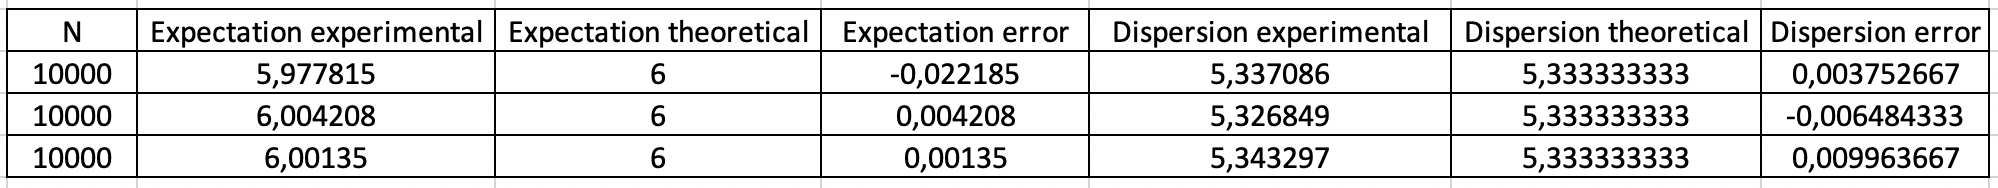
\includegraphics[scale = 0.49]{uniform/1.png}
				\caption{Результаты для равномерного распределения}
			\end{figure}
		\end{center}
		
		\begin{figure}[!htb]
		    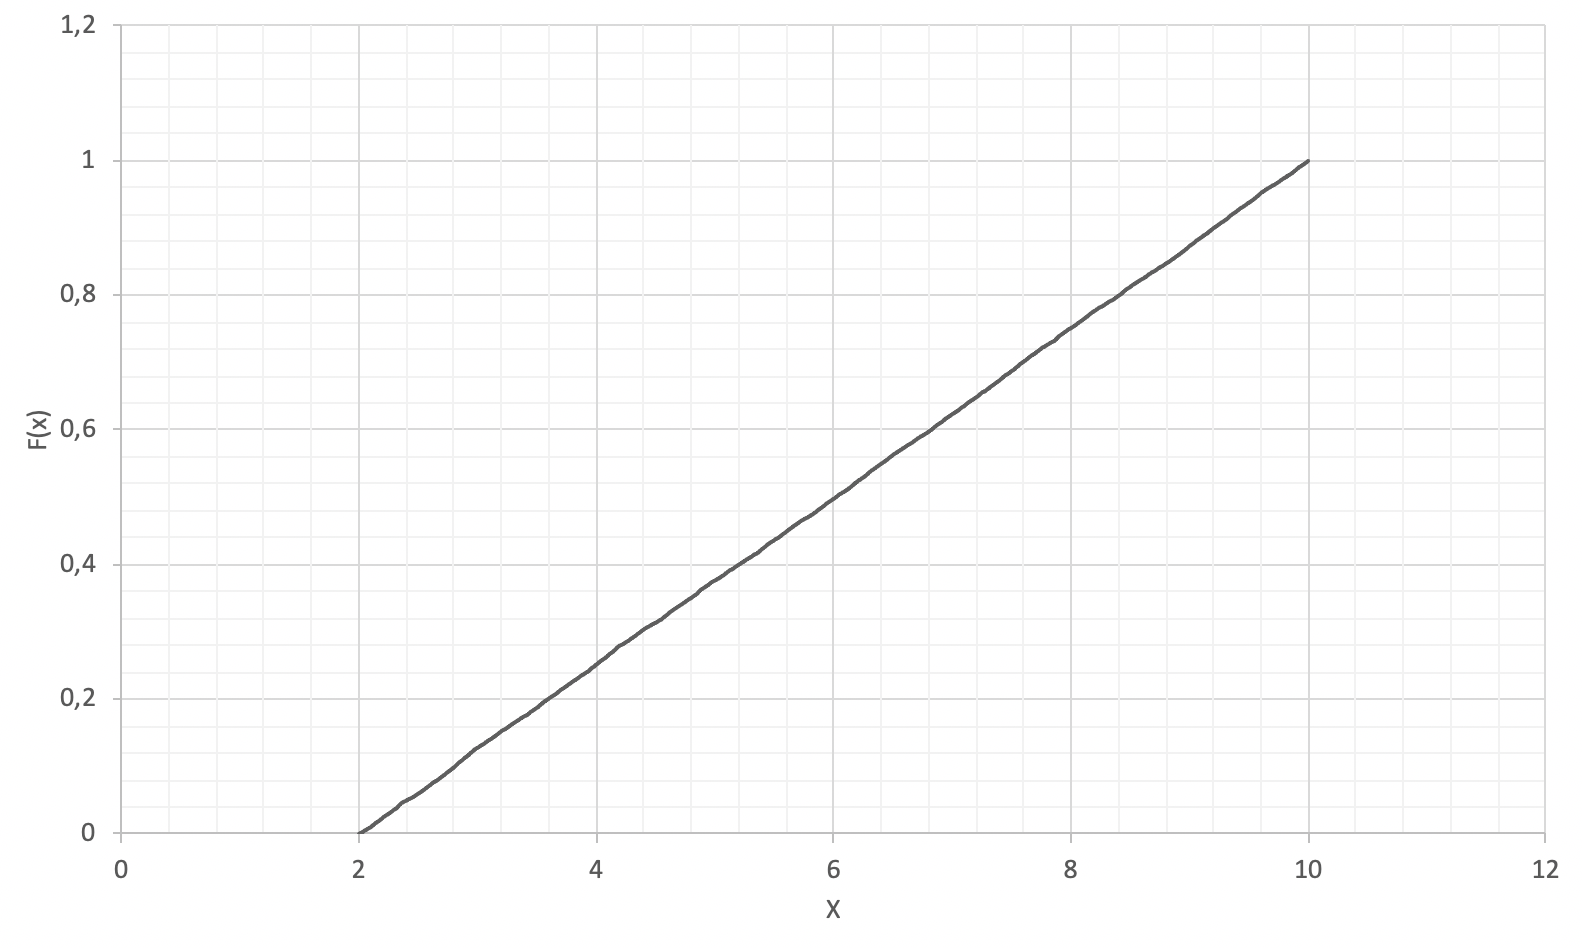
\includegraphics[scale = 0.4]{uniform/2.png}
    		\caption{Функция распределения}
		\end{figure}
		 	 	
		\begin{figure}[!htb]
			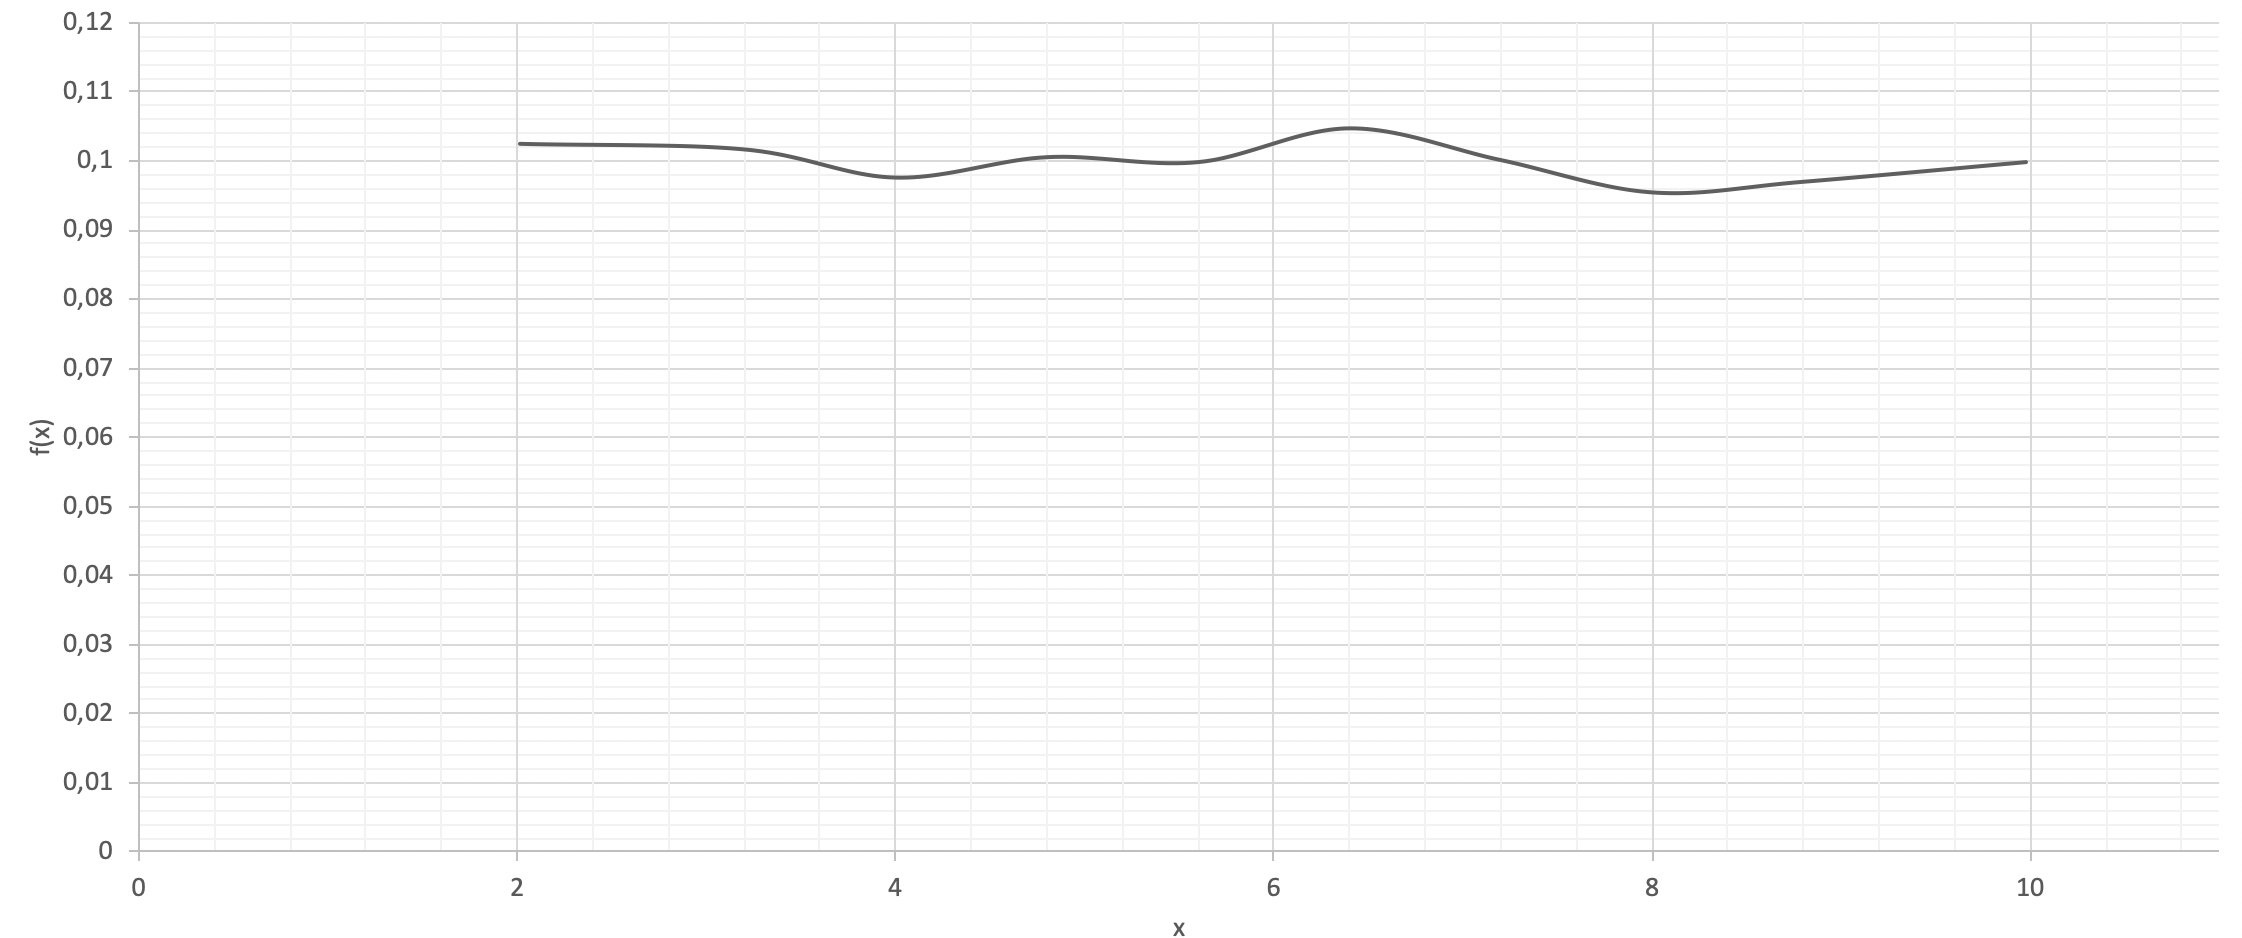
\includegraphics[scale = 0.3]{uniform/3.png}
			\caption{Плотность вероятности}
   		\end{figure}
   	\newpage
										
	%----------------------------------------------------------------------------------------
	%	SECTION 4
	%----------------------------------------------------------------------------------------
	\section{Нормальное распределение}
		Тестирование проводилось на выборке объемом $n = 10000$ значений и параметрами нормального закона распределения
		\begin{center}
			$\mu = -2$\\ 
			$\sigma^2 = 6.25$\\
		\end{center}
		\begin{center}
			\begin{figure}[!htb]
				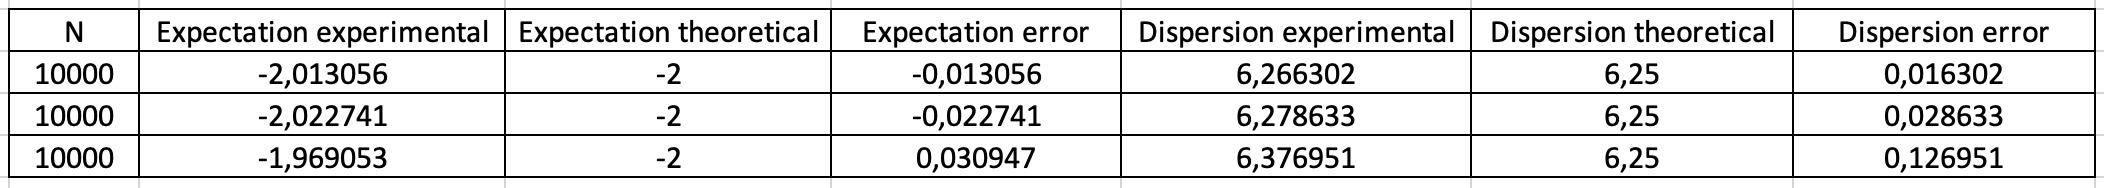
\includegraphics[scale = 0.5]{normal/1.png}
				\caption{Результаты для нормального распределения}
			\end{figure}
		\end{center}
		
		\begin{figure}[!htb]
		    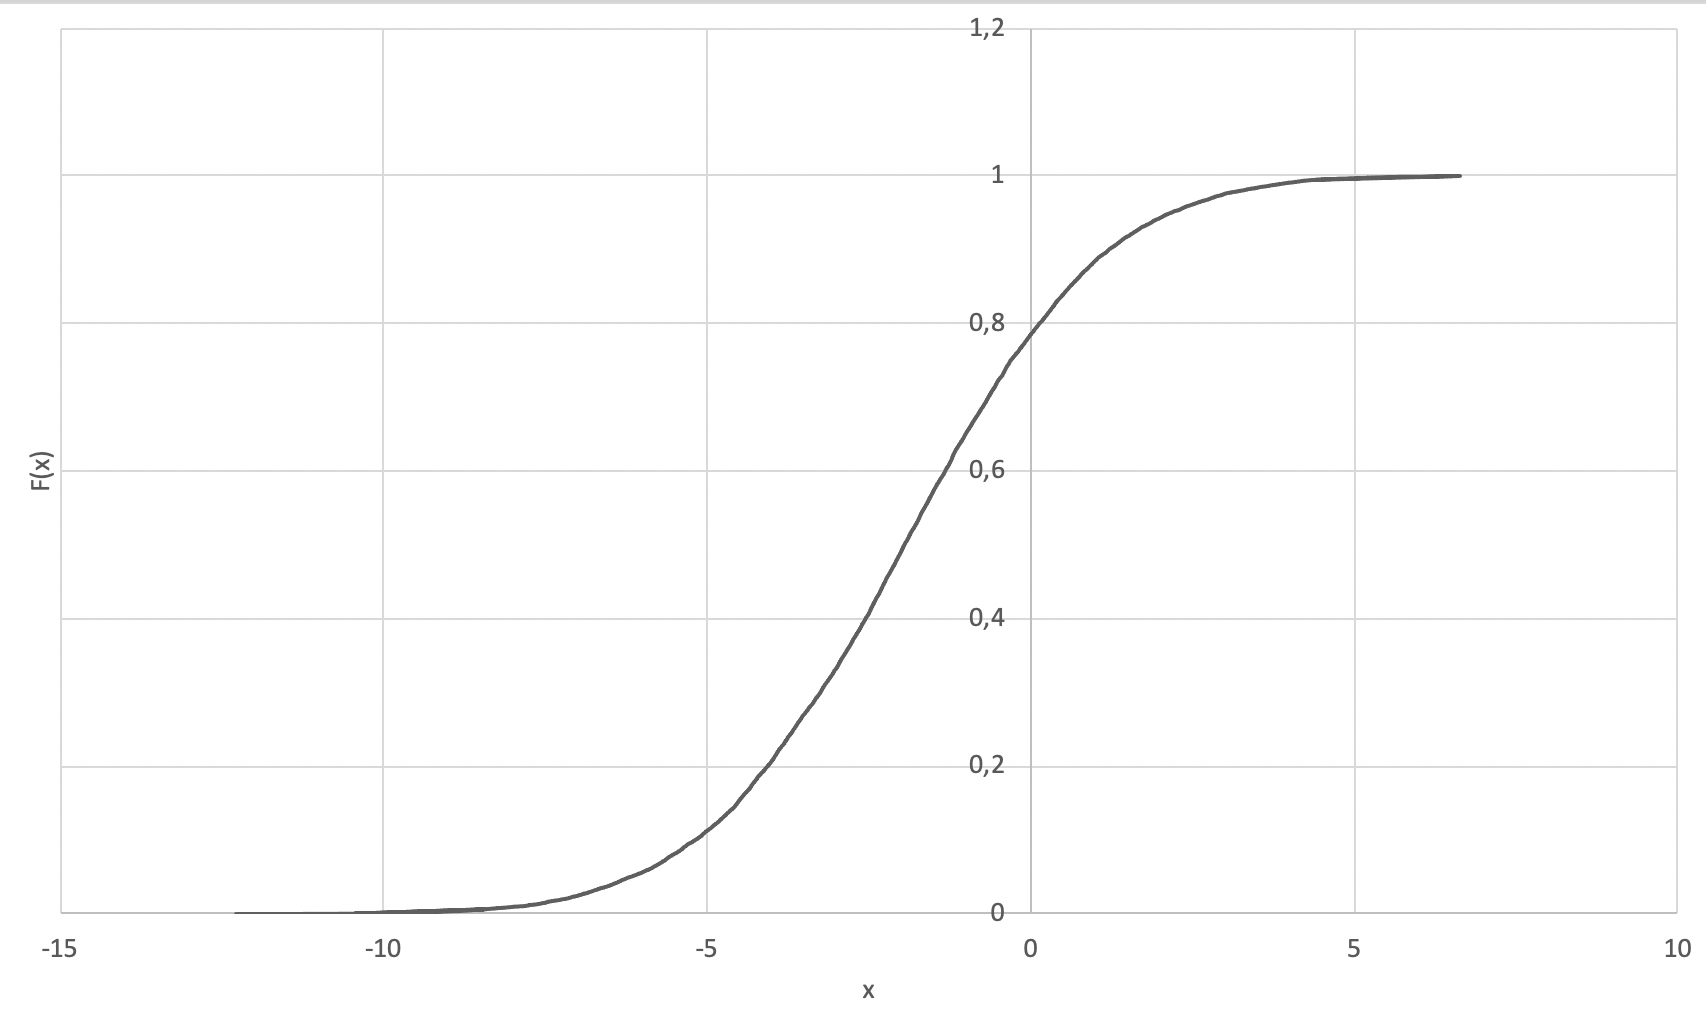
\includegraphics[scale = 0.38]{normal/2.png}
    		\caption{Функция распределения}
		\end{figure}
		 	 	
		\begin{figure}[!htb]
			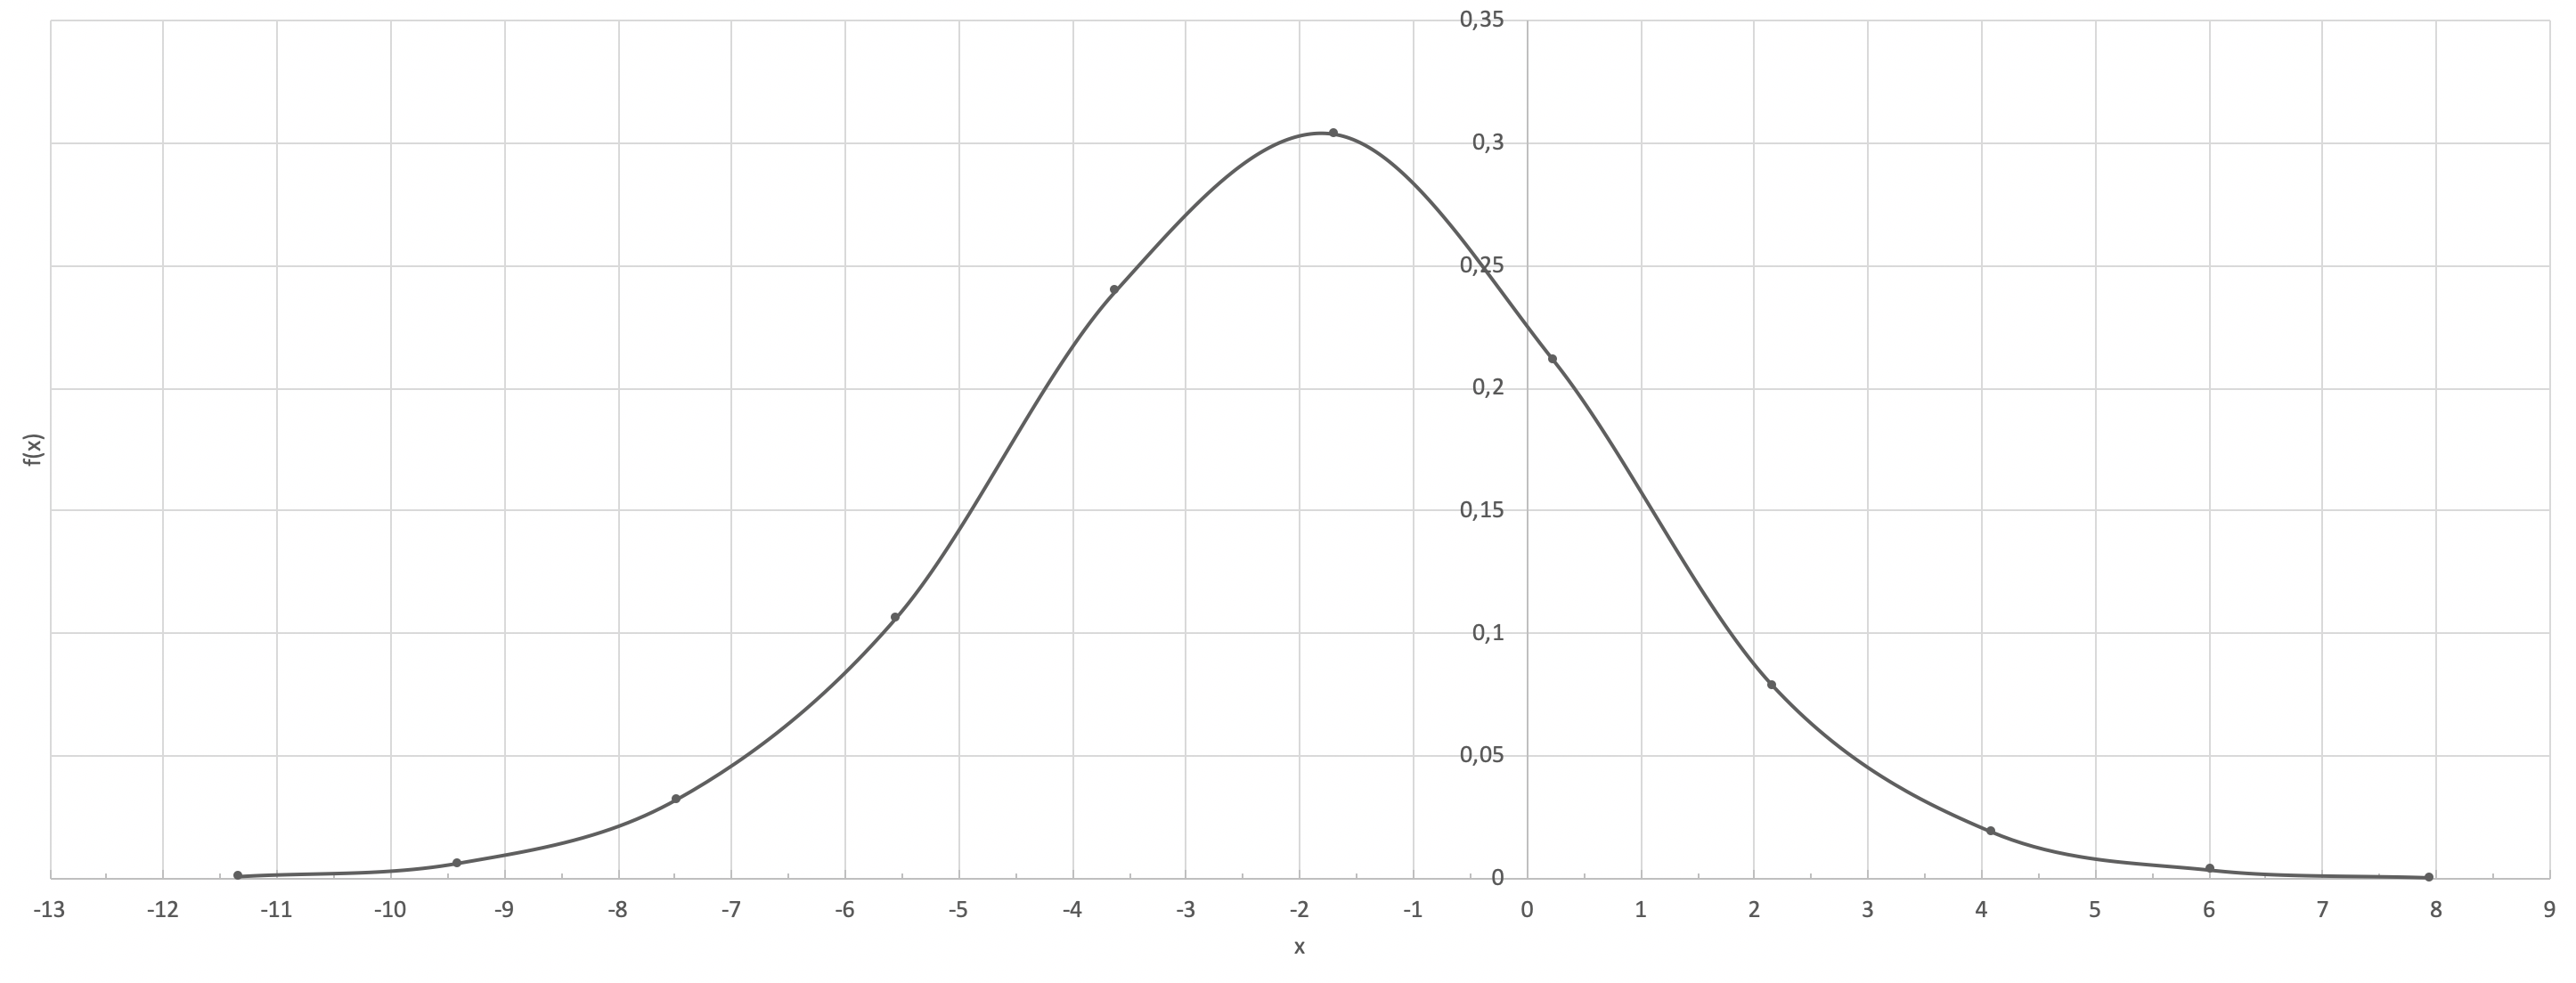
\includegraphics[scale = 0.32]{normal/3.png}
			\caption{Плотность вероятности}
   		\end{figure}
	\newpage

	%----------------------------------------------------------------------------------------
	%	SECTION 5
	%----------------------------------------------------------------------------------------
	\section{Экспоненциальное распределение}
		Тестирование проводилось на выборке объемом $n = 10000$ значений и параметрами экспоненциального закона распределения
		\begin{center}
			$\lambda = 1.5$\\
		\end{center}
		\begin{center}
			\begin{figure}[!htb]
				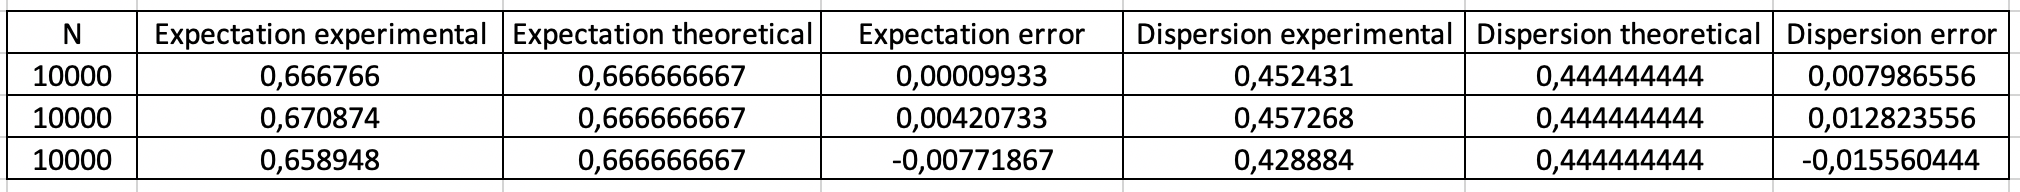
\includegraphics[scale = 0.51]{exp/1.png}
				\caption{Результаты для экспоненциального распределения}
			\end{figure}
		\end{center}
		
		\begin{figure}[!htb]
		    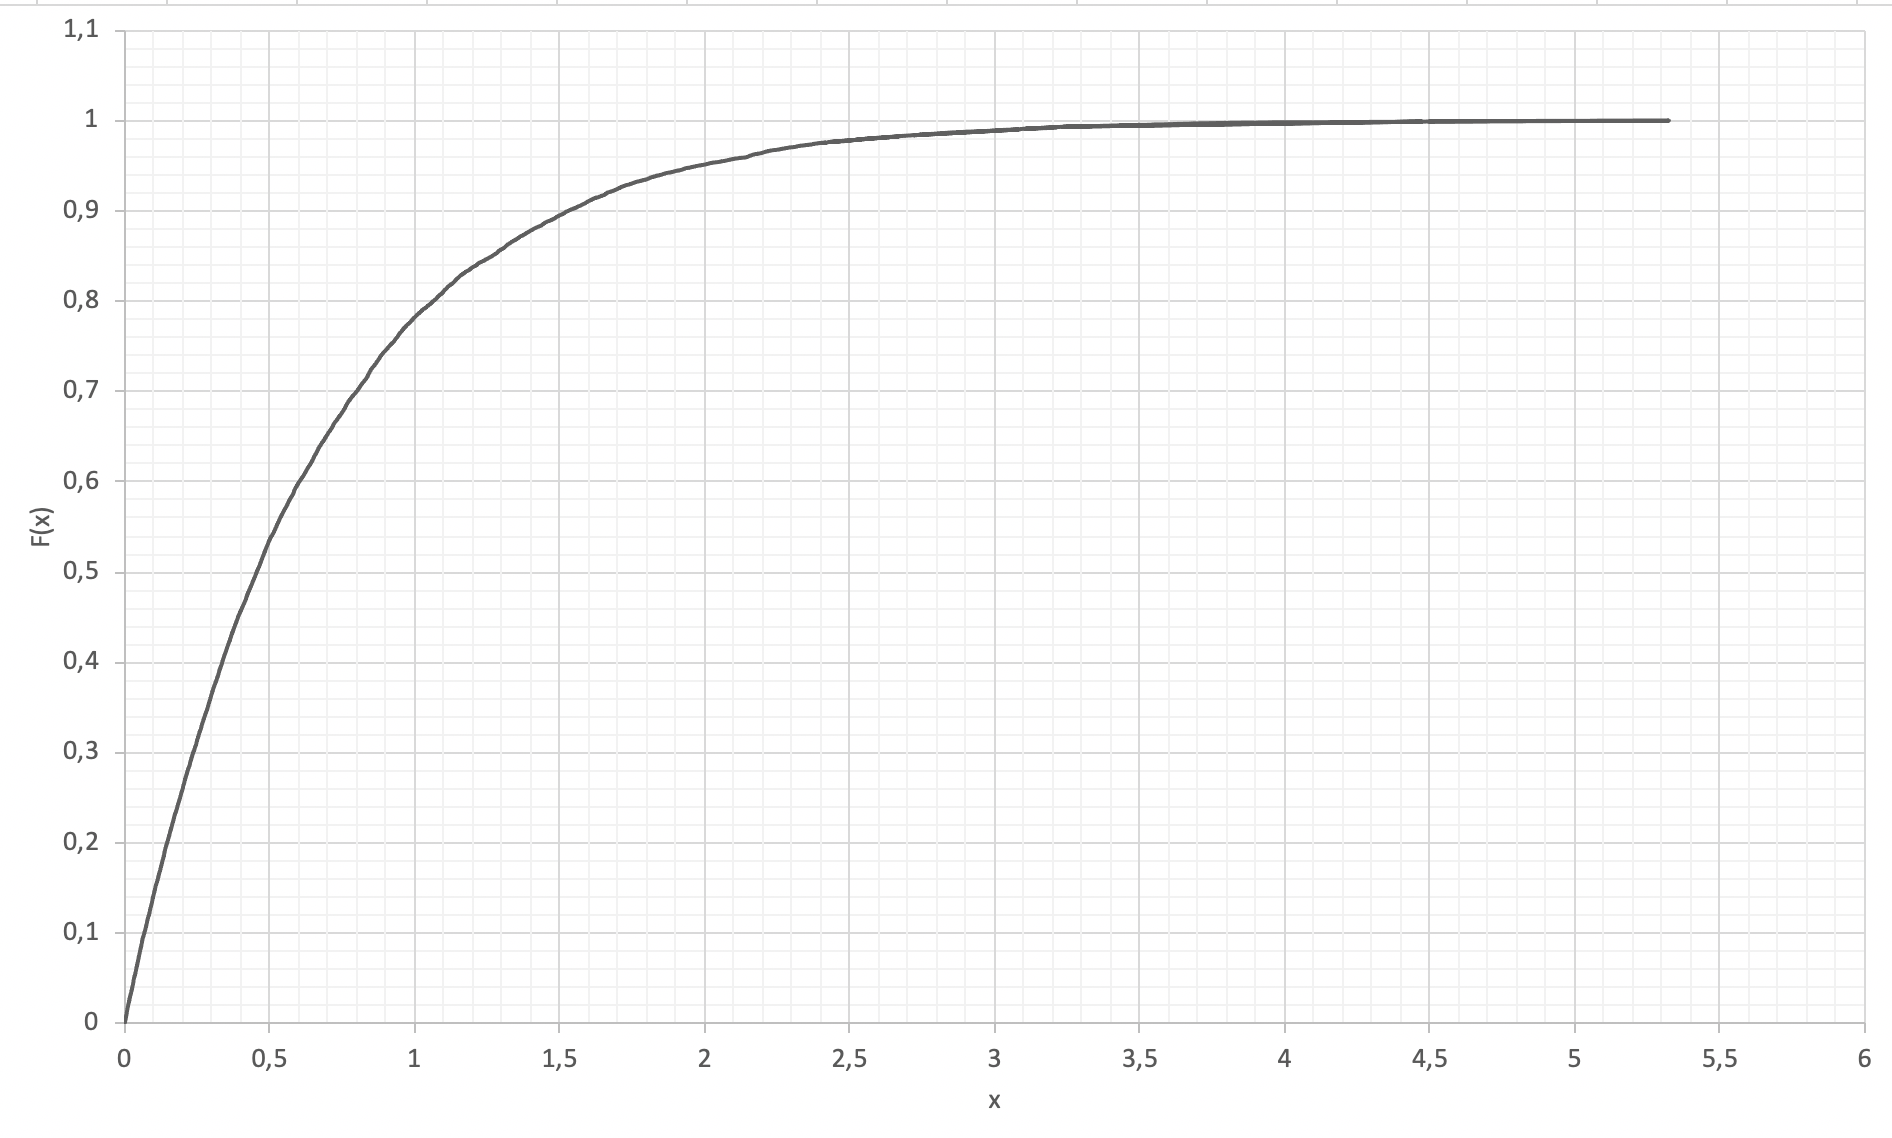
\includegraphics[scale = 0.34]{exp/2.png}
    		\caption{Функция распределения}
		\end{figure}
		 	 	
		\begin{figure}[!htb]
			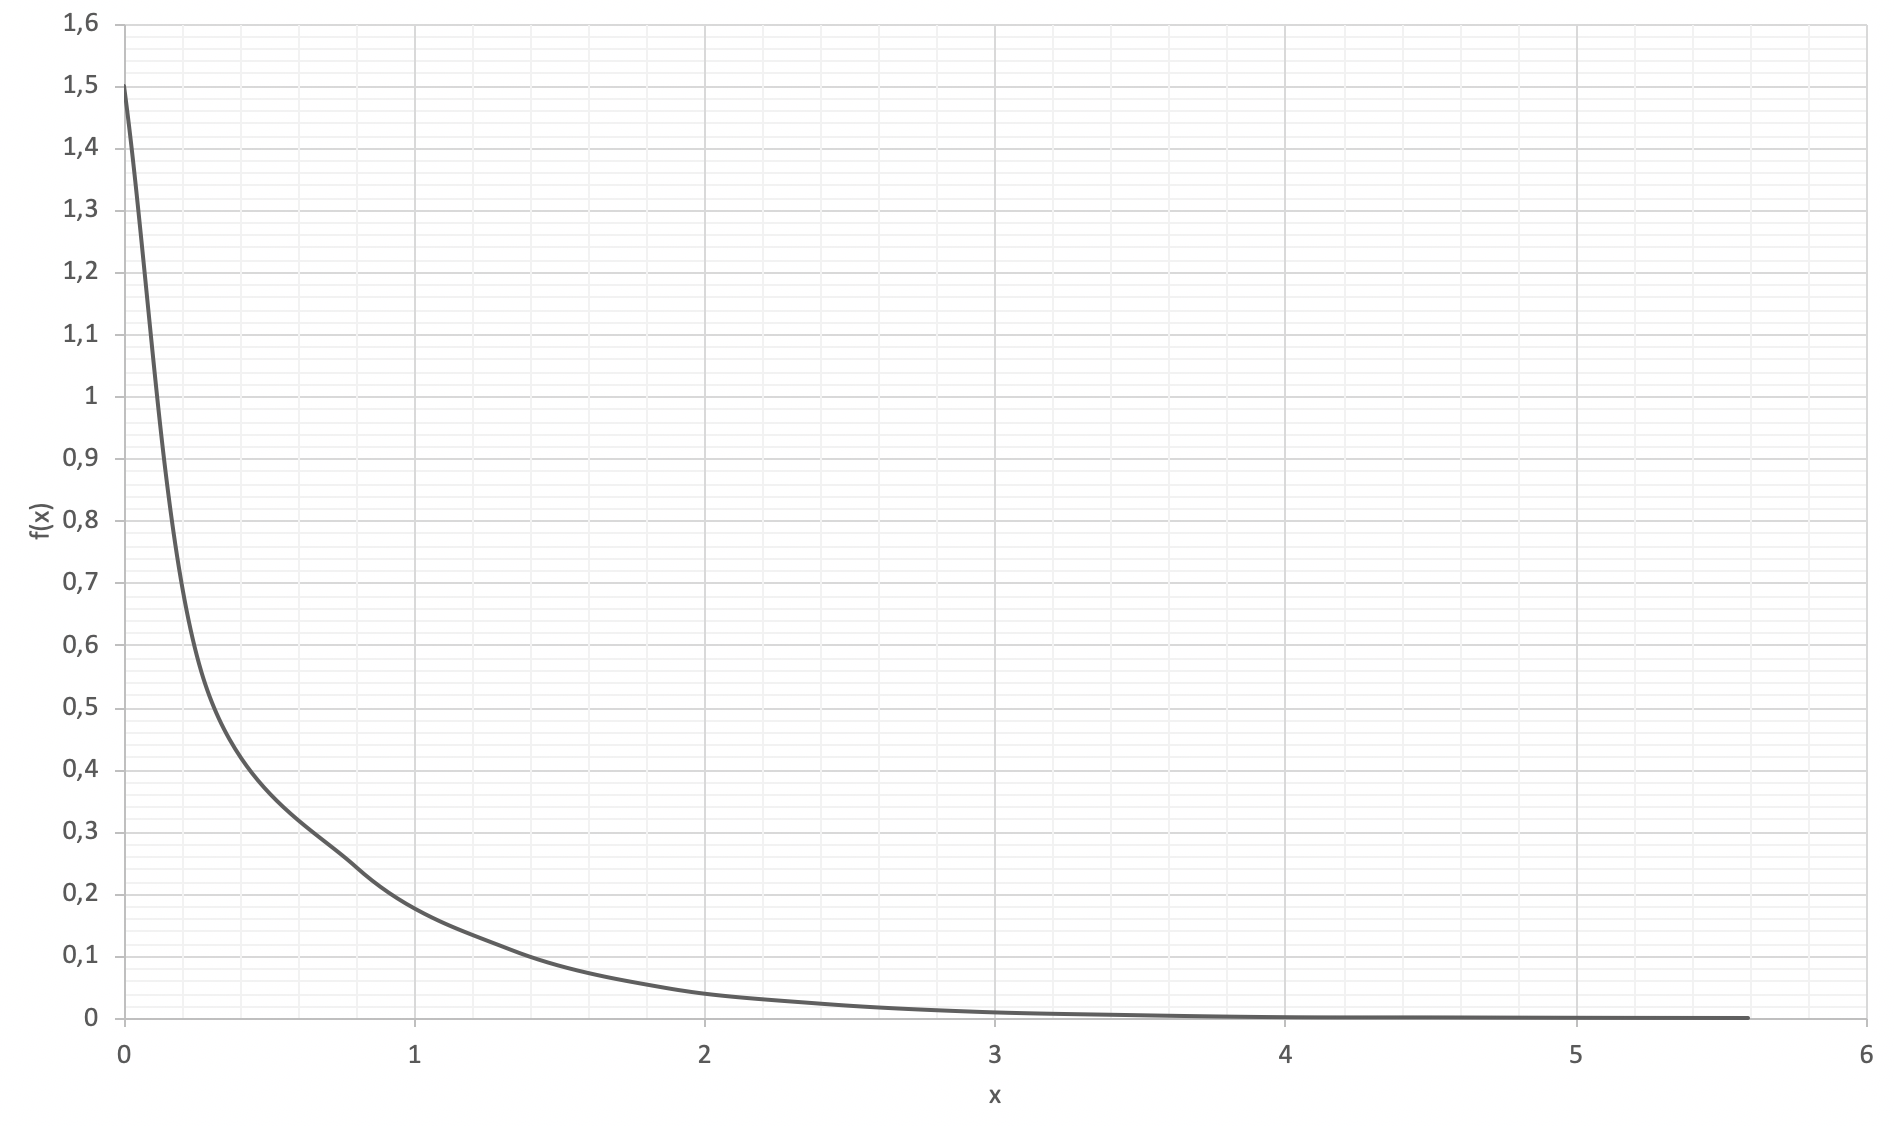
\includegraphics[scale = 0.32]{exp/3.png}
			\caption{Плотность вероятности}
   		\end{figure}
   	\newpage
	
	%----------------------------------------------------------------------------------------
	%	SECTION 6
	%----------------------------------------------------------------------------------------
	\section{Хи-квадрат распределение}
		Тестирование проводилось на выборке объемом $n = 10000$ значений и параметрами закона распределения хи-квадрат
		\begin{center}
			$k = 3$\\
		\end{center}
		\begin{center}
			\begin{figure}[!htb]
				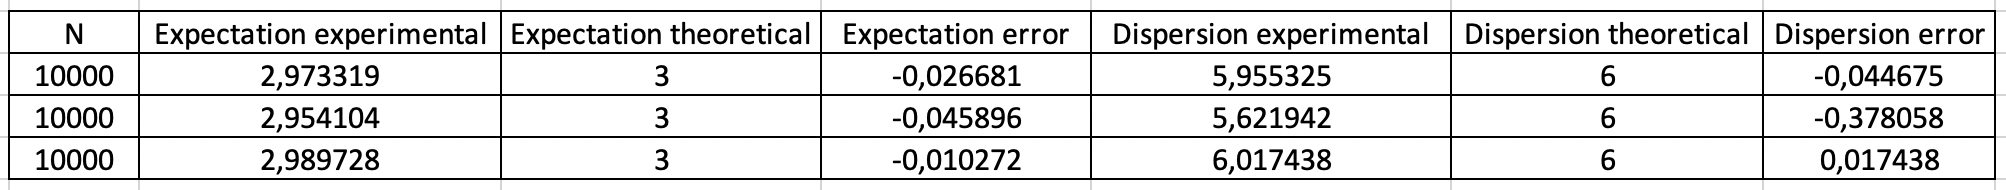
\includegraphics[scale = 0.51]{chisq/1.png}
				\caption{Результаты для распределения хи-кавадрат}
			\end{figure}
		\end{center}
		
		\begin{figure}[!htb]
		    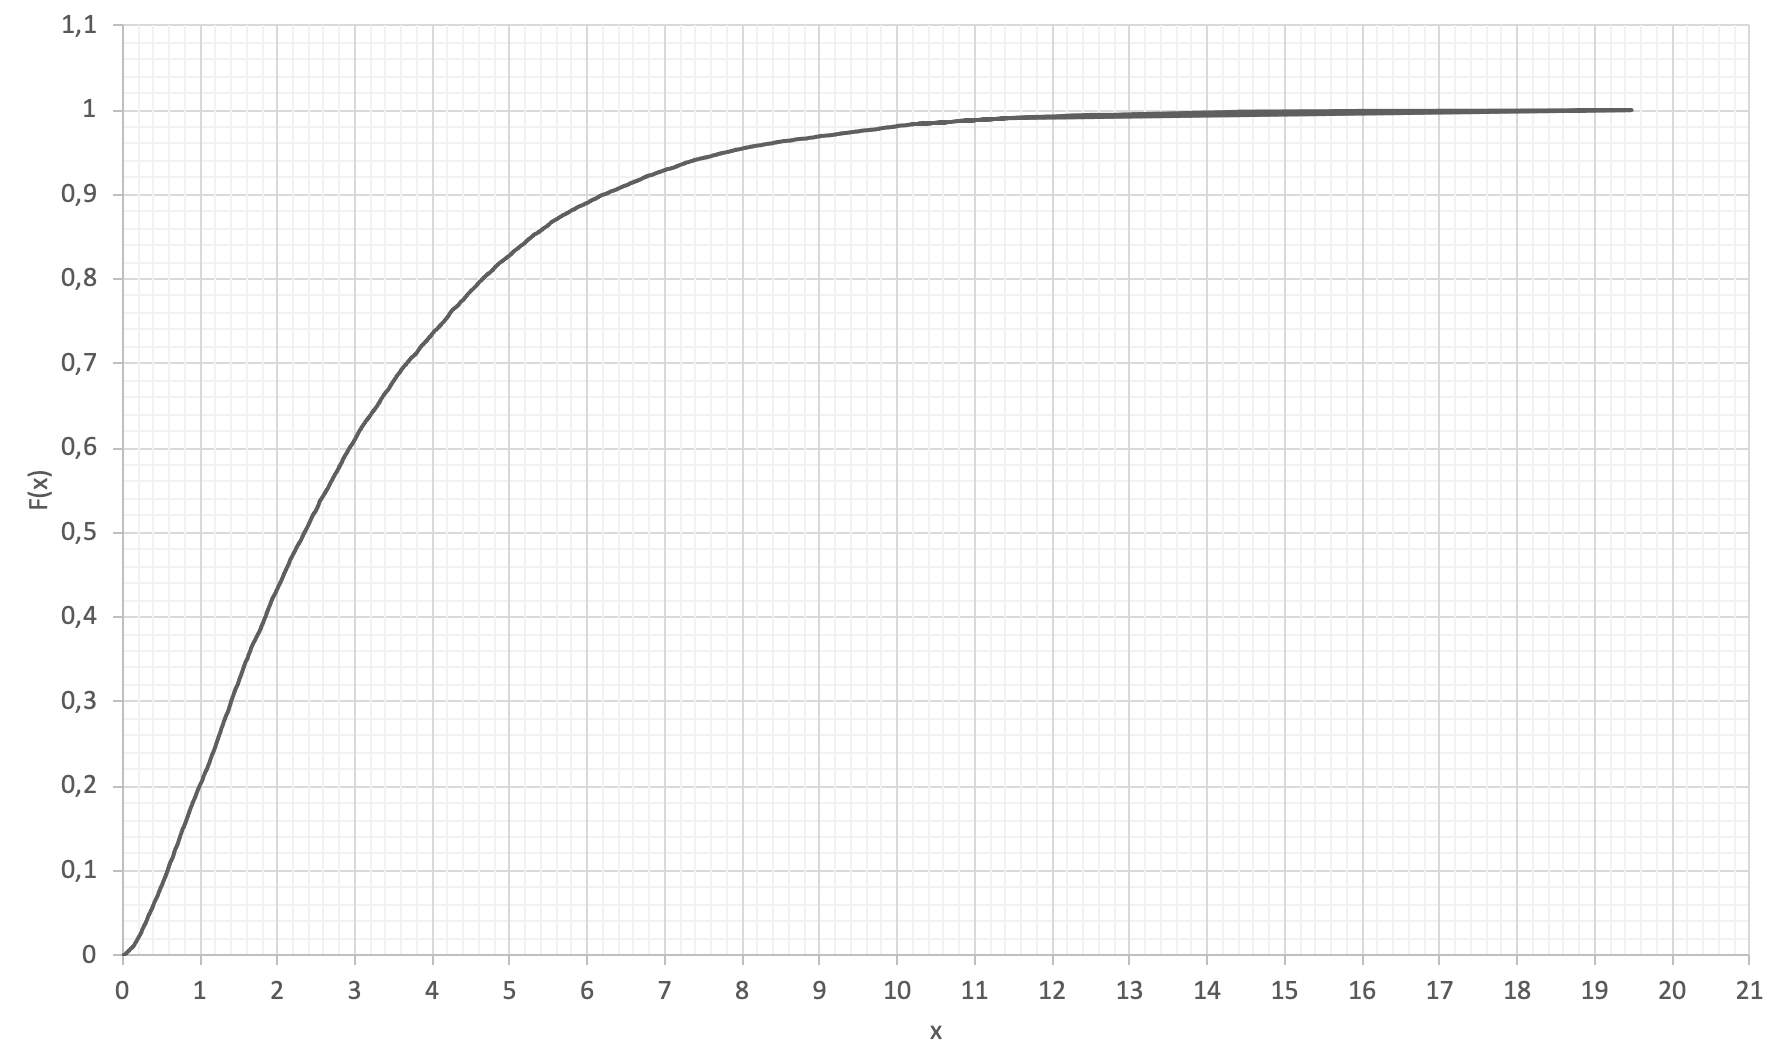
\includegraphics[scale = 0.35]{chisq/2.png}
    		\caption{Функция распределения}
		\end{figure}
		 	 	
		\begin{figure}[!htb]
			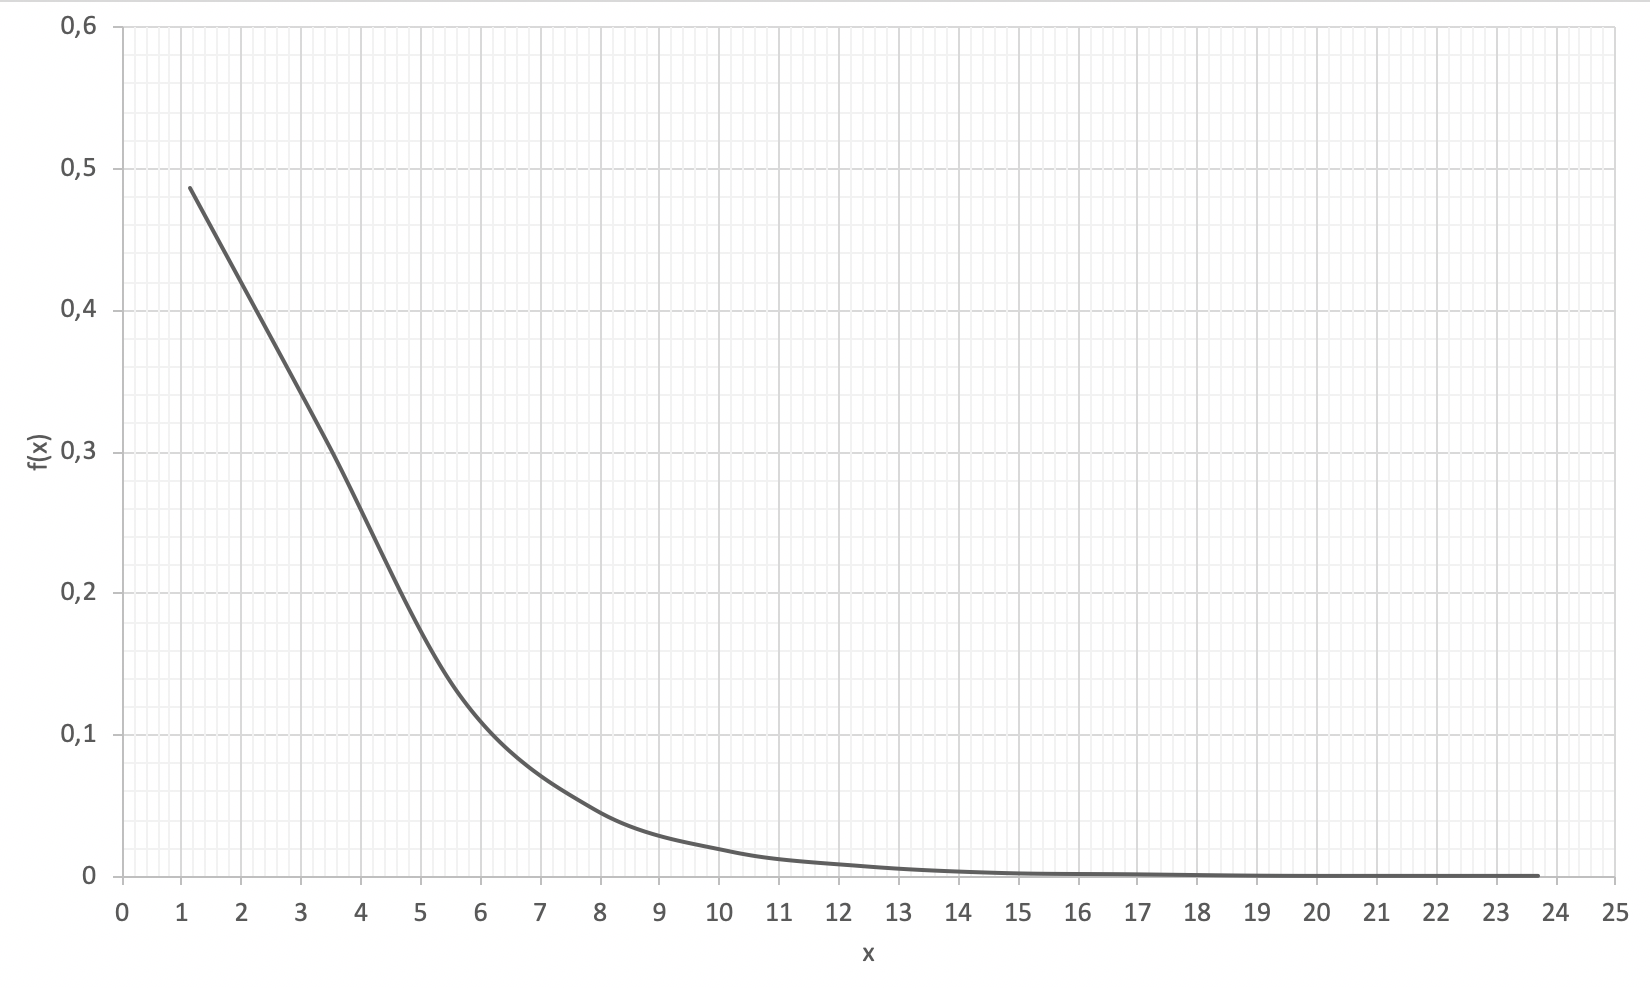
\includegraphics[scale = 0.38]{chisq/3.png}
			\caption{Плотность вероятности}
   		\end{figure}
   	\newpage
   	
   	%----------------------------------------------------------------------------------------
	%	SECTION 7
	%----------------------------------------------------------------------------------------
	\section{Распределение Стьюдента}
		Тестирование проводилось на выборке объемом $n = 10000$ значений и параметрами закона распределения Стьюдента
		\begin{center}
			$k = 5$\\
		\end{center}
		\begin{center}
			\begin{figure}[!htb]
				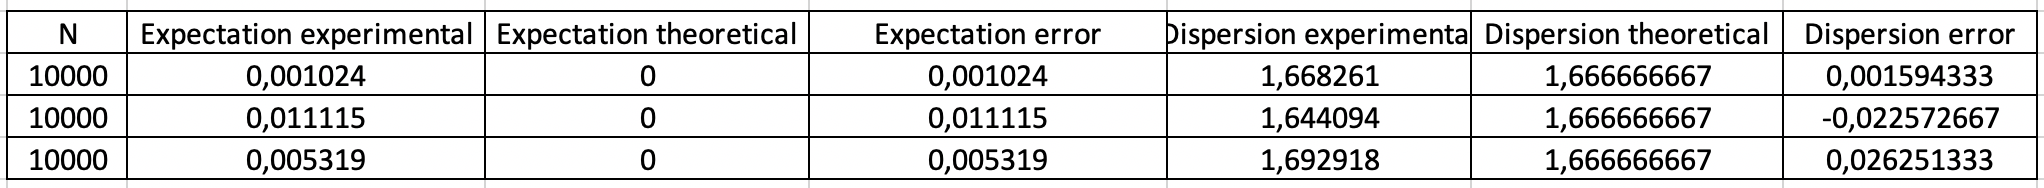
\includegraphics[scale = 0.51]{student/1.png}
				\caption{Результаты для распределения Стьюдента}
			\end{figure}
		\end{center}
		
		\begin{figure}[!htb]
		    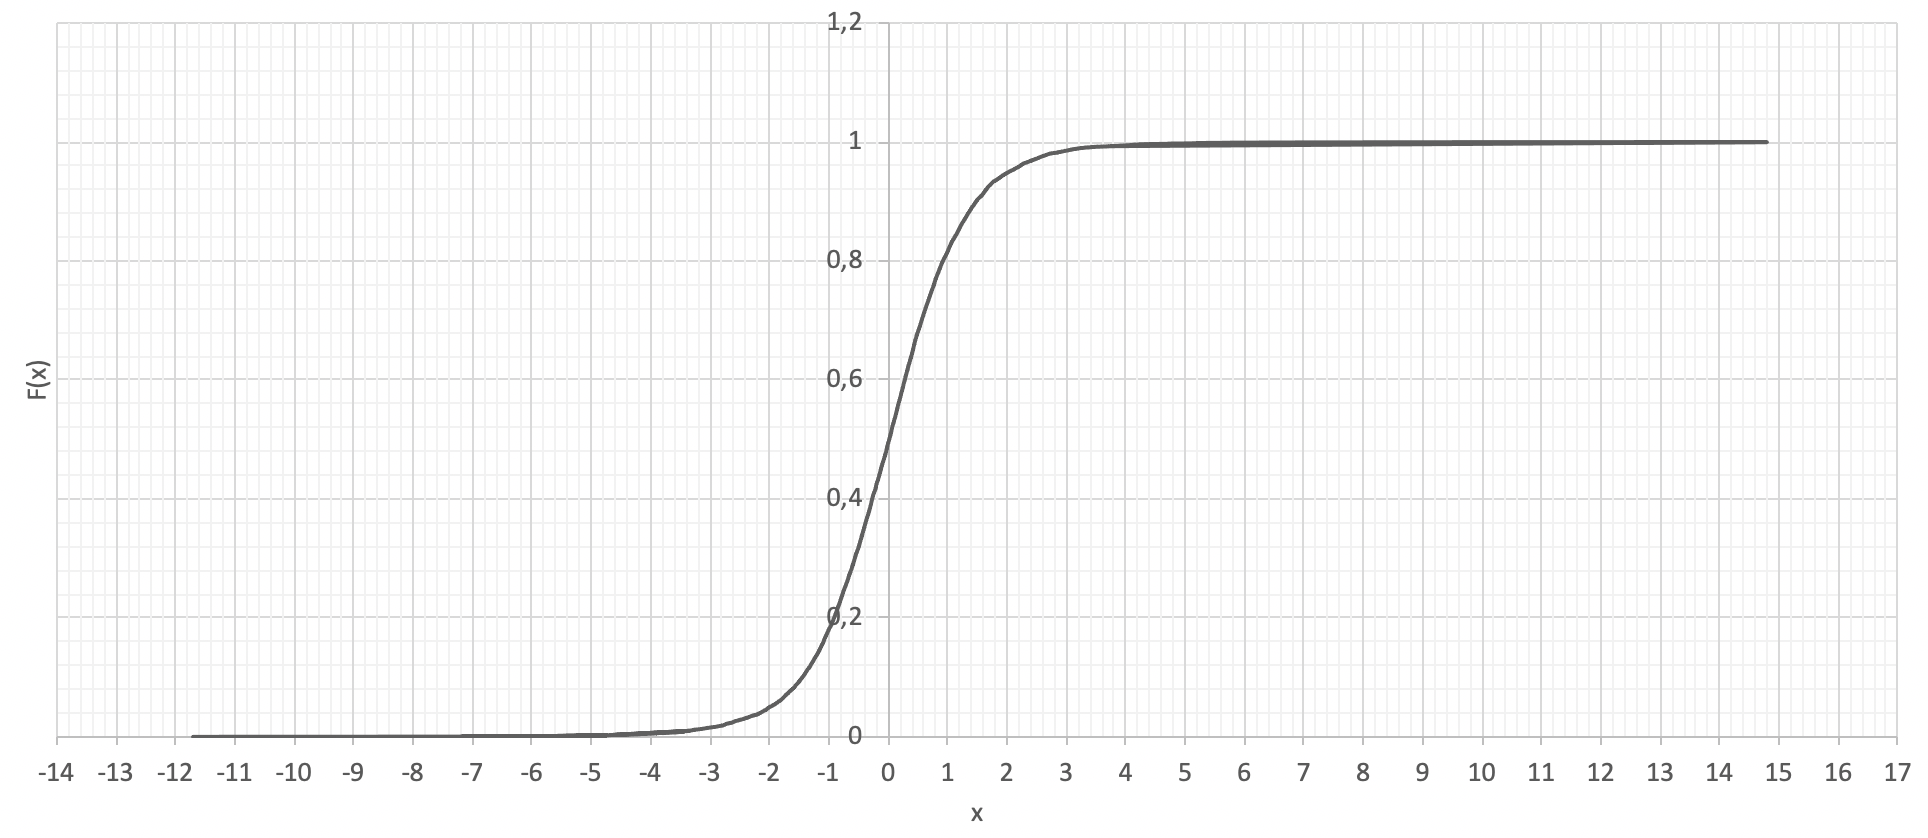
\includegraphics[scale = 0.35]{student/2.png}
    		\caption{Функция распределения}
		\end{figure}
		 	 	
		\begin{figure}[!htb]
			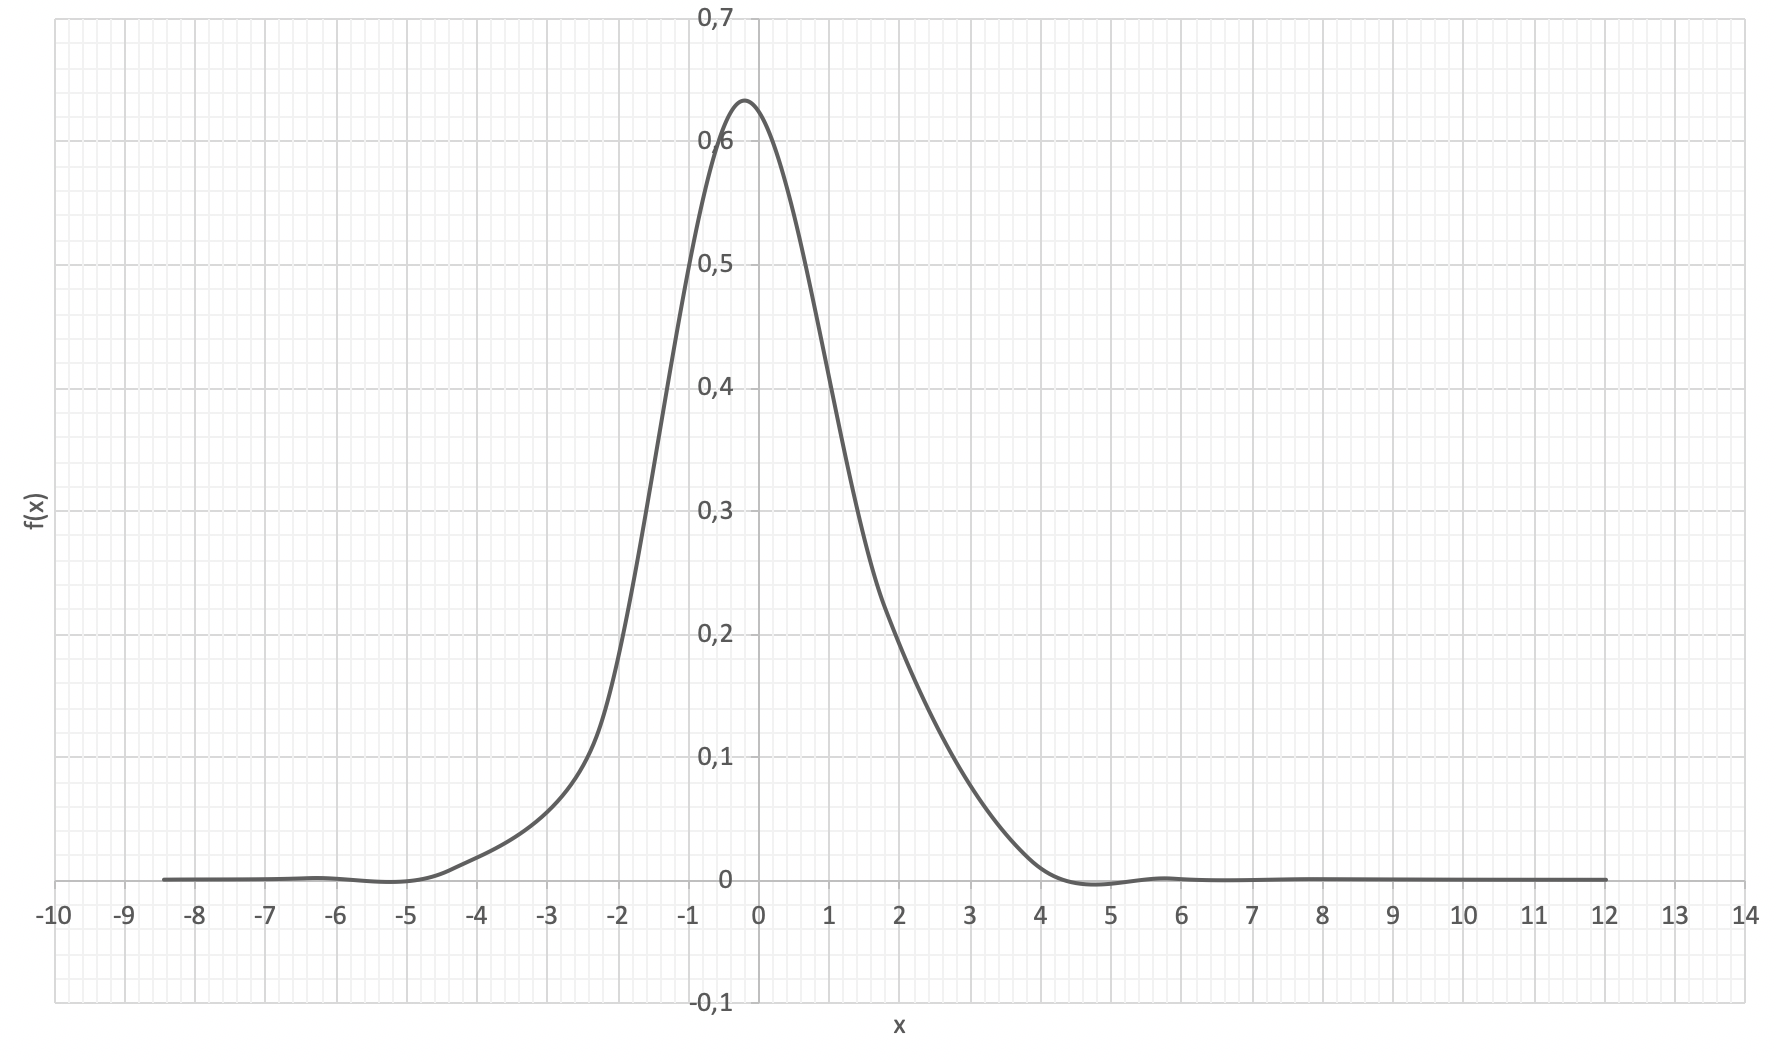
\includegraphics[scale = 0.38]{student/3.png}
			\caption{Плотность вероятности}
   		\end{figure}
   	\newpage

   	%----------------------------------------------------------------------------------------
	%	SECTION 8
	%----------------------------------------------------------------------------------------
   	\section{Вывод}
		В результате проделанной работы были разработаны программные датчики непрерывных случайных величин. Для них были 
		получены мат. ожидание и дисперсия для которых было проведено сравнение с теоретическими значениями. Также были 
		построены графики функции плотности распределения и интегральной функции распределения.	
		Все значенья находятся в рамках небольшой погрешности и соответствуют теоретическим.
	\newpage
	
	%----------------------------------------------------------------------------------------
	%	SECTION 9
	%----------------------------------------------------------------------------------------
   	\section{Приложение}
   		\subsection{Код на языке С++}
   			\lstinputlisting[caption = writer.hpp]{../../src/labs/lab1/model.hpp}
			\lstinputlisting[caption = writer.hpp]{../../src/labs/lab1/writer.hpp}
			\lstinputlisting[caption = main.cpp]{../../src/labs/lab1/main.cpp}
	
	
\end{document}